%!TEX root = ../plos_template.tex

\section*{Four cycle example}

For the purposes of this example, we take the full set of genes to be $L = \{ l_1,l_2,l_3,l_4 \}$. Consider the case in which each of the gene regulatory network modules under consideration has two genes and we specify the covering of the genotype space given by $\mathcal{G} = \{\{l_1,l_2 \},\{l_1,l_4 \},\{l_3,l_2\},\{l_3,l_4\} \}$.  We will compute $\mathbb{L}(\mathcal{G})$ using the same method which was used for the example of three genes.  By analogy with \ref{eq:localconsistencythreegenes}, the local consistency conditions now are as follows:
\begin{equation}
\begin{aligned}\label{eq:pparsys}
p^1_0 &= p^{12}_{00} + p^{12}_{01} = p^{14}_{00} + p^{14}_{01}, &
p^1_1 &= p^{12}_{10} + p^{12}_{11} = p^{14}_{10} + p^{14}_{11},\\
p^3_0 &= p^{32}_{00} + p^{32}_{01} = p^{34}_{00} + p^{34}_{01},&
p^3_1 &= p^{32}_{10} + p^{32}_{11} = p^{34}_{11} + p^{34}_{11},\\
p^2_0 &= p^{12}_{00} + p^{12}_{10} = p^{32}_{00} + p^{32}_{10},&
p^2_1 &= p^{12}_{01} + p^{12}_{11} = p^{32}_{01} + p^{32}_{11},\\
p^4_0 &= p^{14}_{00} + p^{14}_{10} = p^{34}_{00} + p^{34}_{10},&
p^4_1 &= p^{14}_{01} + p^{14}_{11} = p^{34}_{01} + p^{34}_{11}.
\end{aligned}
\end{equation}
Likewise, the equations determined by the conditions $v = \mathbf{G}(x)$ which are analogous to the matrix $\mathbf{G}$ in \ref{fig:efunctor}B are now
\begin{equation}
\begin{aligned}\label{eq:globsys}
p^{12}_{00} &= p^{1234}_{0000} + p^{1234}_{0010} + p^{1234}_{0001} + p^{1234}_{0011} &
p^{12}_{10} &= p^{1234}_{1000} + p^{1234}_{1010} + p^{1234}_{1001} + p^{1234}_{1011} \\
p^{12}_{01} &= p^{1234}_{0100} + p^{1234}_{0110} + p^{1234}_{0101} + p^{1234}_{0111} &
p^{12}_{11} &= p^{1234}_{1100} + p^{1234}_{1110} + p^{1234}_{1101} + p^{1234}_{1111} \\
p^{14}_{00} &= p^{1234}_{0000} + p^{1234}_{0001} + p^{1234}_{1000} + p^{1234}_{1001} &
p^{14}_{10} &= p^{1234}_{0010} + p^{1234}_{0011} + p^{1234}_{1010} + p^{1234}_{1011} \\
p^{14}_{01} &= p^{1234}_{0100} + p^{1234}_{0101} + p^{1234}_{1100} + p^{1234}_{1101} &
p^{14}_{11} &= p^{1234}_{0110} + p^{1234}_{0111} + p^{1234}_{1110} + p^{1234}_{1111} \\
p^{32}_{00} &= p^{1234}_{0000} + p^{1234}_{0010} + p^{1234}_{0100} + p^{1234}_{0110} &
p^{32}_{10} &= p^{1234}_{1000} + p^{1234}_{1010} + p^{1234}_{1100} + p^{1234}_{1110} \\
p^{32}_{01} &= p^{1234}_{0001} + p^{1234}_{0011} + p^{1234}_{0101} + p^{1234}_{0111} &
p^{32}_{11} &= p^{1234}_{1001} + p^{1234}_{1011} + p^{1234}_{1101} + p^{1234}_{1111}\\
p^{34}_{00} &= p^{1234}_{0000} + p^{1234}_{1000} + p^{1234}_{0100} + p^{1234}_{1100} &
p^{34}_{10} &= p^{1234}_{0010} + p^{1234}_{1010} + p^{1234}_{0110} + p^{1234}_{1110} \\
p^{34}_{01} &= p^{1234}_{0001} + p^{1234}_{1001} + p^{1234}_{0101} + p^{1234}_{1101} &
p^{34}_{11} &= p^{1234}_{0011} + p^{1234}_{1011} + p^{1234}_{0111} + p^{1234}_{1111},
\end{aligned}
\end{equation}
which are displayed in matrix form in \ref{tab:logmat222}.

Rather than proceeding to compute $\mathbb{L}(\mathcal{G})$ using elimination of inequalities as before, we will instead make use of the fact that the extremal points of $\mathbb{L}(\mathcal{G})$ happen to be the extremal points of $\mathbb{L}(\mathcal{G})$ with integer coordinates.  This is the approach which was used to compute the volume ratios shown in \ref{fig:ncycvolrat}.  More specifically, those computations were done using a computer program based on the following algorithm which is available via a virtual machine that can be reconstructed using the instructions available on \href{https://github.com/cameronraysmith/sep}{github}:

\begin{enumerate}
\item Compute (a basis for) the cokernel of $\mathbf{G}$. The cokernel gives the obstructions to the system $\mathbf{G}\mathbf{X}=\mathbf{V}$ having a solution. In order to eliminate these obstructions constraints must be imposed on $\mathbb{R}^{\mathcal{E}(\mathcal{G})}$ and these constraints are given precisely via annihilating the cokernel.
\item Use the constraints on $\mathbb{R}^{\mathcal{E}(\mathcal{G})}$ from step 1 necessary for the system $\mathbf{G}\mathbf{X}=\mathbf{V}$ to have a solution to eliminate variables from the system of inequalities $\mathbf{V} \geq 0$ giving a half-space representation or H-representation of the polytope $\mathbb{L}(\mathcal{G})$. This can be used to compute $\text{Vol}(\mathbb{L}(\mathcal{G}))$.
\item Compute the vertices of $\mathbb{L}(\mathcal{G})$ from the H-representation determined in step 2 giving a vertex representation or V-representation of $\mathbb{L}(\mathcal{G})$.
\item Filter the non-integer rational vertices from the collection computed in step 3 to produce a corresponding V-representation of $\mathbb{M}(\mathcal{G})$ \cite{Wainwright2007} proposition 8.3.
\item Compute $\text{Vol}(\mathbb{M}(\mathcal{G}))$ from the V-represention of $\mathbb{M}(\mathcal{G})$.
\end{enumerate}

For standard computations on polytopes, we make use of the standard algorithms incorporated by the polymake project \cite{Gawrilow2000}. In some cases, the volume computation is too costly to perform exactly. In those cases we use the approximation given in \cite{Cousins}.  We now return to our example of four genes $\mathcal{G} = \{\{l_1,l_2 \},\{l_1,l_4 \},\{l_3,l_2\},\{l_3,l_4\} \}$ and $P=\{0,1\}$ and use it to walk through key components of the algorithm.

The equalities derived by computing the cokernel of the matrix $\mathbf{G}$ given in \ref{tab:logmat222} and adjoining rows that enforce the normalization of the marginal distributions are represented as a matrix in \ref{eq:eqmat}.
\begin{equation}\label{eq:eqmat}
\begin{aligned}
\begin{bmatrix}
  -1 & -1 & 0 & 0 & 1 & 1 & 0 & 0 & 0 & 0 & 0 & 0 & 0 & 0 & 0 & 0 & 0\\
  0 & 0 & -1 & -1 & 0 & 0 & 1 & 1 & 0 & 0 & 0 & 0 & 0 & 0 & 0 & 0 & 0\\
  -1 & 0 & -1 & 0 & 0 & 0 & 0 & 0 & 1 & 1 & 0 & 0 & 0 & 0 & 0 & 0 & 0\\
  0 & -1 & 0 & -1 & 0 & 0 & 0 & 0 & 0 & 0 & 1 & 1 & 0 & 0 & 0 & 0 & 0\\
  0 & 0 & 0 & 0 & 0 & 0 & 0 & 0 & -1 & 0 & -1 & 0 & 1 & 1 & 0 & 0 & 0\\
  0 & 0 & 0 & 0 & -1 & 0 & -1 & 0 & 0 & 0 & 0 & 0 & 1 & 0 & 1 & 0 & 0\\
  -1 & -1 & -1 & -1 & 1 & 0 & 1 & 0 & 1 & 0 & 1 & 0 & -1 & 0 & 0 & 1 & 0\\
  1 & 1 & 1 & 1 & 0 & 0 & 0 & 0 & 0 & 0 & 0 & 0 & 0 & 0 & 0 & 0 & 1\\
  0 & 0 & 0 & 0 & 1 & 1 & 1 & 1 & 0 & 0 & 0 & 0 & 0 & 0 & 0 & 0 & 1\\
  0 & 0 & 0 & 0 & 0 & 0 & 0 & 0 & 1 & 1 & 1 & 1 & 0 & 0 & 0 & 0 & 1\\
  0 & 0 & 0 & 0 & 0 & 0 & 0 & 0 & 0 & 0 & 0 & 0 & 1 & 1 & 1 & 1 & 1\\
\end{bmatrix}
\end{aligned}
\end{equation}
The final column represents the right-hand side of each equality. It turns out all but one of the normalization conditions is linearly dependent with respect to the other equalities and so we can reduce this set of $7+4=11$ constraints to the $8$ represented again in matrix form in \ref{eq:kceqsrefa}.
\begin{equation}\label{eq:kceqsrefa}
\begin{aligned}
\begin{bmatrix}
  1 & 0 & 0 & -1 & 0 & 0 & 1 & 1 & 0 & 0 & 1 & 1 & 0 & 0 & 0 & 0 & 1\\
  0 & 1 & 0 & 1 & 0 & 0 & 0 & 0 & 0 & 0 & -1 & -1 & 0 & 0 & 0 & 0 & 0\\
  0 & 0 & 1 & 1 & 0 & 0 & -1 & -1 & 0 & 0 & 0 & 0 & 0 & 0 & 0 & 0 & 0\\
  0 & 0 & 0 & 0 & 1 & 0 & 1 & 0 & 0 & 0 & 0 & 0 & 0 & 1 & 0 & 1 & 1\\
  0 & 0 & 0 & 0 & 0 & 1 & 0 & 1 & 0 & 0 & 0 & 0 & 0 & -1 & 0 & -1 & 0\\
  0 & 0 & 0 & 0 & 0 & 0 & 0 & 0 & 1 & 0 & 1 & 0 & 0 & 0 & 1 & 1 & 1\\
  0 & 0 & 0 & 0 & 0 & 0 & 0 & 0 & 0 & 1 & 0 & 1 & 0 & 0 & -1 & -1 & 0\\
  0 & 0 & 0 & 0 & 0 & 0 & 0 & 0 & 0 & 0 & 0 & 0 & 1 & 1 & 1 & 1 & 1\\
\end{bmatrix}
\end{aligned}
\end{equation}
These equalities can now be substituted into the positivity inequalities necessary to define any space of probability distributions. This yields a set of inequalities \ref{eq:polrepindineqs} that specify an H-representation of the polytope $\mathbb{L}(\mathcal{G})$. This is the modular polytope, which is a subspace of $\Delta_3^{\oplus 4}$ associated to distributions consistent with the linear transformation $\mathbf{G}$
\begin{equation}\label{eq:polrepindineqs}
\begin{aligned}
\begin{bmatrix}
  1 & 1 & -1 & -1 & -1 & -1 & 0 & 0 & 0\\
  0 & -1 & 0 & 0 & 1 & 1 & 0 & 0 & 0\\
  0 & -1 & 1 & 1 & 0 & 0 & 0 & 0 & 0\\
  1 & 0 & -1 & 0 & 0 & 0 & -1 & 0 & -1\\
  0 & 0 & 0 & -1 & 0 & 0 & 1 & 0 & 1\\
  1 & 0 & 0 & 0 & -1 & 0 & 0 & -1 & -1\\
  0 & 0 & 0 & 0 & 0 & -1 & 0 & 1 & 1\\
  1 & 0 & 0 & 0 & 0 & 0 & -1 & -1 & -1\\
  0 & 1 & 0 & 0 & 0 & 0 & 0 & 0 & 0\\
  0 & 0 & 1 & 0 & 0 & 0 & 0 & 0 & 0\\
  0 & 0 & 0 & 1 & 0 & 0 & 0 & 0 & 0\\
  0 & 0 & 0 & 0 & 1 & 0 & 0 & 0 & 0\\
  0 & 0 & 0 & 0 & 0 & 1 & 0 & 0 & 0\\
  0 & 0 & 0 & 0 & 0 & 0 & 1 & 0 & 0\\
  0 & 0 & 0 & 0 & 0 & 0 & 0 & 1 & 0\\
  0 & 0 & 0 & 0 & 0 & 0 & 0 & 0 & 1\\
\end{bmatrix}
\end{aligned}
\end{equation}
A row $(a_0,a_1,...,a_d)$ corresponds to the inequality $a_0 + a_1 x_1 + ... + a_d x_d >= 0$. The embedded identity matrix has, in this particular case eight, rows that specify the positivity of the variables corresponding to each of the, in this particular case eight, dimensions. Transforming this inequality or H-representation to a vertex or V-representation of the modular polytope produces \ref{eq:vrepfromhrep}.
\begin{equation}\label{eq:vrepfromhrep}
\begin{aligned}
\begin{bmatrix}
  1 & 0 & 0 & 0 & 0 & 0 & 0 & 0 & 1\\
  1 & 0 & 0 & 0 & 0 & 0 & 0 & 1 & 0\\
  1 & 0 & 0 & 0 & 0 & 0 & 1 & 0 & 0\\
  1 & 1/2 & 1/2 & 0 & 1/2 & 0 & 1/2 & 1/2 & 0\\
  1 & 1/2 & 0 & 1/2 & 0 & 1/2 & 1/2 & 1/2 & 0\\
  1 & 0 & 0 & 0 & 0 & 0 & 0 & 0 & 0\\
  1 & 1/2 & 1/2 & 0 & 0 & 1/2 & 0 & 0 & 1/2\\
  1 & 1/2 & 0 & 1/2 & 1/2 & 0 & 0 & 0 & 1/2\\
  1 & 0 & 0 & 1/2 & 0 & 1/2 & 0 & 0 & 1/2\\
  1 & 0 & 1/2 & 0 & 1/2 & 0 & 0 & 0 & 1/2\\
  1 & 0 & 1/2 & 0 & 0 & 1/2 & 1/2 & 1/2 & 0\\
  1 & 0 & 0 & 1/2 & 1/2 & 0 & 1/2 & 1/2 & 0\\
  1 & 1 & 1 & 0 & 1 & 0 & 0 & 0 & 0\\
  1 & 0 & 0 & 0 & 1 & 0 & 0 & 0 & 0\\
  1 & 0 & 1 & 0 & 0 & 0 & 0 & 0 & 0\\
  1 & 0 & 0 & 1 & 0 & 0 & 1 & 0 & 0\\
  1 & 0 & 0 & 0 & 0 & 1 & 0 & 1 & 0\\
  1 & 0 & 0 & 0 & 1 & 0 & 1 & 0 & 0\\
  1 & 0 & 1 & 0 & 0 & 0 & 0 & 1 & 0\\
  1 & 1 & 0 & 1 & 0 & 1 & 0 & 0 & 1\\
  1 & 1 & 0 & 1 & 1 & 0 & 1 & 0 & 0\\
  1 & 1 & 1 & 0 & 0 & 1 & 0 & 1 & 0\\
  1 & 0 & 0 & 1 & 0 & 0 & 0 & 0 & 1\\
  1 & 0 & 0 & 0 & 0 & 1 & 0 & 0 & 1\\
\end{bmatrix}
\end{aligned}
\end{equation}
This completes steps 1-3 of the algorithm outlined above. Step 4 is trivial; to obtain the V-represention of $\mathbb{M}(\mathcal{G})$, we strike out the rows in which $1/2$ appears.  Finally, we compute the volume of the polytope whose vertices are the rows of \ref{eq:vrepfromhrep} to obtain $\text{Vol}(\mathbb{L}(\mathcal{G})) = \frac{1}{120}$ and the volume of the polytope whose vertices are rows of integers to obtain $\text{Vol}(\mathbb{M}(\mathcal{G})) = \frac{1}{180}$ yielding a ratio $\frac{\text{Vol}(\mathbb{M}(\mathcal{G}))}{\text{Vol}(\mathbb{L}(\mathcal{G}))} = \frac{2}{3}$.

% \section{A generative process for apparently inconsistent pairwise distributions}\label{sec:generativeprocessapparentinconsistency}

% The inequalities defining $\mathbb{M}(\mathcal{G})$ were derived under the assumption that the two-element probabilities were obtained by mariginalizing a three-element distribution.  Hence, if some other procedure, such as conditionalization is used to obtain them instead, the inequalities need not apply, as in the example above, which may be described as follows:  Introduce the sample spaces
% \begin{align*}
% S_{1} &= \{e_0,e_1\} \\
% S_{2} &= \{f_0,f_1\} \\
% S_{3} &= \{g_0,g_1\} \\
% S_{12} &= \{b_{00},b_{01},b_{10},b_{11}\} \\
% S_{13} &= \{c_{00},c_{01},c_{10},c_{11}\} \\
% S_{23} &= \{d_{00},d_{01},d_{10},d_{11}\} \\
% S_{123} &= \{a_{002},a_{012},a_{102},a_{112},a_{020},a_{021},a_{120},a_{121},a_{200},a_{201},a_{210},a_{211}\}, \\
% \end{align*}
% the inclusion maps $\iota_1, \iota_2, \iota_3$ and the projections $\pi_1, \ldots. \pi_6$.
% $$
% \xymatrix{
% S_{1}& S_{13} \ar@{->>}[l]_{\pi_1} \ar@{->>}[r]^{\pi_2} \ar@{^{(}->}[d]_{\iota_2} & S_{3} \\
% S_{12} \ar@{->>}[u]^{\pi_3} \ar@{->>}[rd]_{\pi_5} \ar@{^{(}->}[r]^{\iota_1} & S_{123} & S_{23} \ar@{->>}[u]^{\pi_4} \ar@{->>}[ld]^{\pi_6} \ar@{_{(}->}[l]_{\iota_3} \\
% & S_2 & }
% $$
% \begin{center}
% \begin{tabular}{c | c}
% $x$ & $\iota_1 (x)$ \\ \hline
% $b_{00}$ & $a_{002}$ \\
% $b_{01}$ & $a_{012}$ \\
% $b_{10}$ & $a_{102}$ \\
% $b_{11}$ & $a_{112}$ \\
% \end{tabular} \qquad
% \begin{tabular}{c | c}
% $x$ & $\iota_2 (x)$ \\ \hline
% $c_{00}$ & $a_{020}$ \\
% $c_{01}$ & $a_{021}$ \\
% $c_{10}$ & $a_{120}$ \\
% $c_{11}$ & $a_{121}$ \\
% \end{tabular} \qquad
% \begin{tabular}{c | c}
% $x$ & $\iota_3 (x)$ \\ \hline
% $d_{00}$ & $a_{200}$ \\
% $d_{01}$ & $a_{201}$ \\
% $d_{10}$ & $a_{210}$ \\
% $d_{11}$ & $a_{211}$ \\
% \end{tabular}
% \end{center}

% \begin{center}
% \begin{tabular}{c | c}
% $x$ & $\pi_1 (x)$ \\ \hline
% $c_{00}$ & $e_0$ \\
% $c_{01}$ & $e_0$ \\
% $c_{10}$ & $e_1$ \\
% $c_{11}$ & $e_1$ \\
% \end{tabular} \quad
% \begin{tabular}{c | c}
% $x$ & $\pi_2 (x)$ \\ \hline
% $c_{00}$ & $g_0$ \\
% $c_{01}$ & $g_1$ \\
% $c_{10}$ & $g_0$ \\
% $c_{11}$ & $g_1$ \\
% \end{tabular} \quad
% \begin{tabular}{c | c}
% $x$ & $\pi_3 (x)$ \\ \hline
% $b_{00}$ & $e_0$ \\
% $b_{01}$ & $e_0$ \\
% $b_{10}$ & $e_1$ \\
% $b_{11}$ & $e_1$ \\
% \end{tabular} \quad
% \begin{tabular}{c | c}
% $x$ & $\pi_4 (x)$ \\ \hline
% $d_{00}$ & $g_0$ \\
% $d_{01}$ & $g_1$ \\
% $d_{10}$ & $g_0$ \\
% $d_{11}$ & $g_1$ \\
% \end{tabular} \quad
% \begin{tabular}{c | c}
% $x$ & $\pi_5 (x)$ \\ \hline
% $b_{00}$ & $f_0$ \\
% $b_{01}$ & $f_1$ \\
% $b_{10}$ & $f_0$ \\
% $b_{11}$ & $f_1$ \\
% \end{tabular} \quad
% \begin{tabular}{c | c}
% $x$ & $\pi_6 (x)$ \\ \hline
% $d_{00}$ & $f_0$ \\
% $d_{01}$ & $f_0$ \\
% $d_{10}$ & $f_1$ \\
% $d_{11}$ & $f_1$ \\
% \end{tabular}
% \end{center}
% \ref{fig:condmargprobspaces} shows these mappings in terms of colored subsets.

% It is thus possible to generate what appear to be inconsistent pairwise distributions by embedding the system in \ref{fig:inconsistentthreecycle} into a consistent system represented by \ref{fig:controlnetwork}. In this system we consider the collection of pairwise probability distributions $p(l_1,l_2)$, $p(l_2,l_3)$, $p(l_1,l_3)$, and the joint probability distribution $p(m_1,m_2,m_3,m_4)$ where the states of genes $l_i \in \{ 0, 1\}$ and genes $m_i \in \{0,1,2\} \equiv \mathcal{M}$. The random variables representing the states of genes $l_1,l_2,l_3$ correspond to $m_1,m_2,m_3$ respectively and $m_4$ is a control random variable colored in dark gray in \ref{fig:controlnetwork}. We specify the control exhibited by $m_4$ over $m_1,m_2,m_3$ via the constraints
% \begin{align*}
% p(m_1=2|m_4=0)=1,\\
% p(m_2=2|m_4=1)=1,\\
% p(m_3=2|m_4=2)=1.
% \end{align*}
% We set $p(l_1,l_2)$, $p(l_2,l_3)$, $p(l_1,l_3)$ equal to those along the respective edges in \ref{fig:inconsistentthreecycle}A and then enforce analogous constraints on $p(m_1,m_2,m_3,m_4)$
% \begin{align*}
% p(m_1,m_2|m_4=2)=p(l_1,l_2),\\
% p(m_2,m_3|m_4=0)=p(l_2,l_3),\\
% p(m_1,m_3|m_4=1)=p(l_1,l_3).
% \end{align*}
% Finally, we place a uniform distribution on the states of $m_4$, $\forall m \in \mathcal{M} \left[ p(m_4=m) = 1/|\mathcal{M}| \right]$. This leads to the joint distribution
% \begin{align*}
% p(m_1,m_2,m_3,m_4=\{0022\})&=1/30,\\
% p(m_1,m_2,m_3,m_4=\{0122\})&=2/15,\\
% p(m_1,m_2,m_3,m_4=\{1022\})&=2/15,\\
% p(m_1,m_2,m_3,m_4=\{1122\})&=1/30,\\
% p(m_1,m_2,m_3,m_4=\{0201\})&=2/15,\\
% p(m_1,m_2,m_3,m_4=\{0211\})&=1/30,\\
% p(m_1,m_2,m_3,m_4=\{1201\})&=1/30,\\
% p(m_1,m_2,m_3,m_4=\{1211\})&=2/15,\\
% p(m_1,m_2,m_3,m_4=\{2000\})&=2/15,\\
% p(m_1,m_2,m_3,m_4=\{2010\})&=1/30,\\
% p(m_1,m_2,m_3,m_4=\{2100\})&=1/30,\\
% p(m_1,m_2,m_3,m_4=\{2110\})&=2/15,
% \end{align*}
% where probabilities for all unlisted states are precisely zero. Now if we compute the conditional distributions
% \begin{align*}
% p(m_1,m_2|m_4=2) = \begin{bmatrix}
% 0.1 & 0.4 & 0\\
% 0.4 & 0.1 & 0\\
% 0 & 0 & 0
% \end{bmatrix},\\
% p(m_2,m_3|m_4=0) = \begin{bmatrix}
% 0.4 & 0.1 & 0\\
% 0.1 & 0.4 & 0\\
% 0 & 0 & 0
% \end{bmatrix},\\
% p(m_1,m_3|m_4=1) = \begin{bmatrix}
% 0.4 & 0.1 & 0\\
% 0.1 & 0.4 & 0\\
% 0 & 0 & 0
% \end{bmatrix},
% \end{align*}
% we see that were we to only observe the variables $m_1,m_2,m_3$ we would arrive at pairwise distributions consistent with
% \begin{align*}
% p(l_1,l_2) = \begin{bmatrix}
% 0.1 & 0.4\\
% 0.4 & 0.1
% \end{bmatrix},\\
% p(l_2,l_3) = \begin{bmatrix}
% 0.4 & 0.1\\
% 0.1 & 0.4
% \end{bmatrix},\\
% p(l_1,l_3) = \begin{bmatrix}
% 0.4 & 0.1\\
% 0.1 & 0.4
% \end{bmatrix},
% \end{align*}
% which cannot derive as marginals from any $p(l_1,l_2,l_3)$.

% % 1--2 conditioned on x_3=3, x_4=3
% %     0.4000    0.1000         0
% %     0.1000    0.4000         0
% %          0         0         0

% % 2--3 conditioned on x_1=3, x_4=1
% %     0.4000    0.1000         0
% %     0.1000    0.4000         0
% %          0         0         0

% % 1--3 conditioned on x_2=3, x_4=2
% %     0.1000    0.4000         0
% %     0.4000    0.1000         0
% %          0         0         0

% This scenario may be implemented via a synthetic gene circuit with four genes, where each of the first three genes contains an operator site for each of the other two and all three genes contain an operator site for the fourth gene \ref{fig:condgenescenario}. If the fourth gene is constitutively expressed at a low rate so that it persists at low copy number it is uniformly, in time, likely to be bound to the operator site present on each of the first three genes. When gene four is bound to its operator site on any of the first three genes, that gene's state is $2$. If gene four is absent, the output state is determined by the presence or absence of the other two operator sites according to each of the tables depicted in \ref{fig:condgenescenario}.

\FloatBarrier
\pagebreak

\begin{figure}[!ht]
\centering
\noindent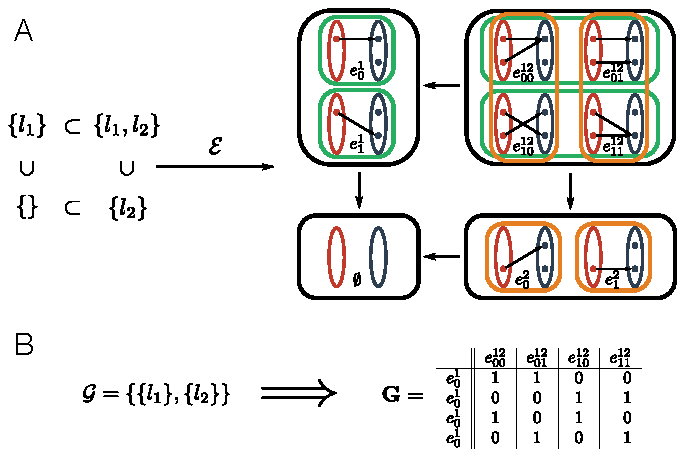
\includegraphics[width=0.8\columnwidth]{fig/efunctor.pdf}
\caption{{\bf Example of the functor mapping subsets of genes to measurable spaces.} (A) On the left hand side are subsets of $L=\{l_1,l_2\}$ ordered by inclusion. On the right hand side are the spaces of gene network-phenotype maps also ordered by inclusion. The labels for the maps define them. For example, $e^{12}_{01}(l_1) = 0$ and $e^{12}_{01}(l_2) = 1$. (B) For the given covering, $\mathcal{G}$, the associated marginalization matrix acting on the probability vector $\{ p^{12}_{00},p^{12}_{01},p^{12}_{10},p^{12}_{11} \}$ to give $\{ p^{1}_{0},p^{1}_{1},p^{2}_{0},p^{2}_{1} \}$ is $\mathbf{G}$.}
\label{fig:efunctor}
\end{figure}

\pagebreak

\begin{figure}[!ht]
\centering
\noindent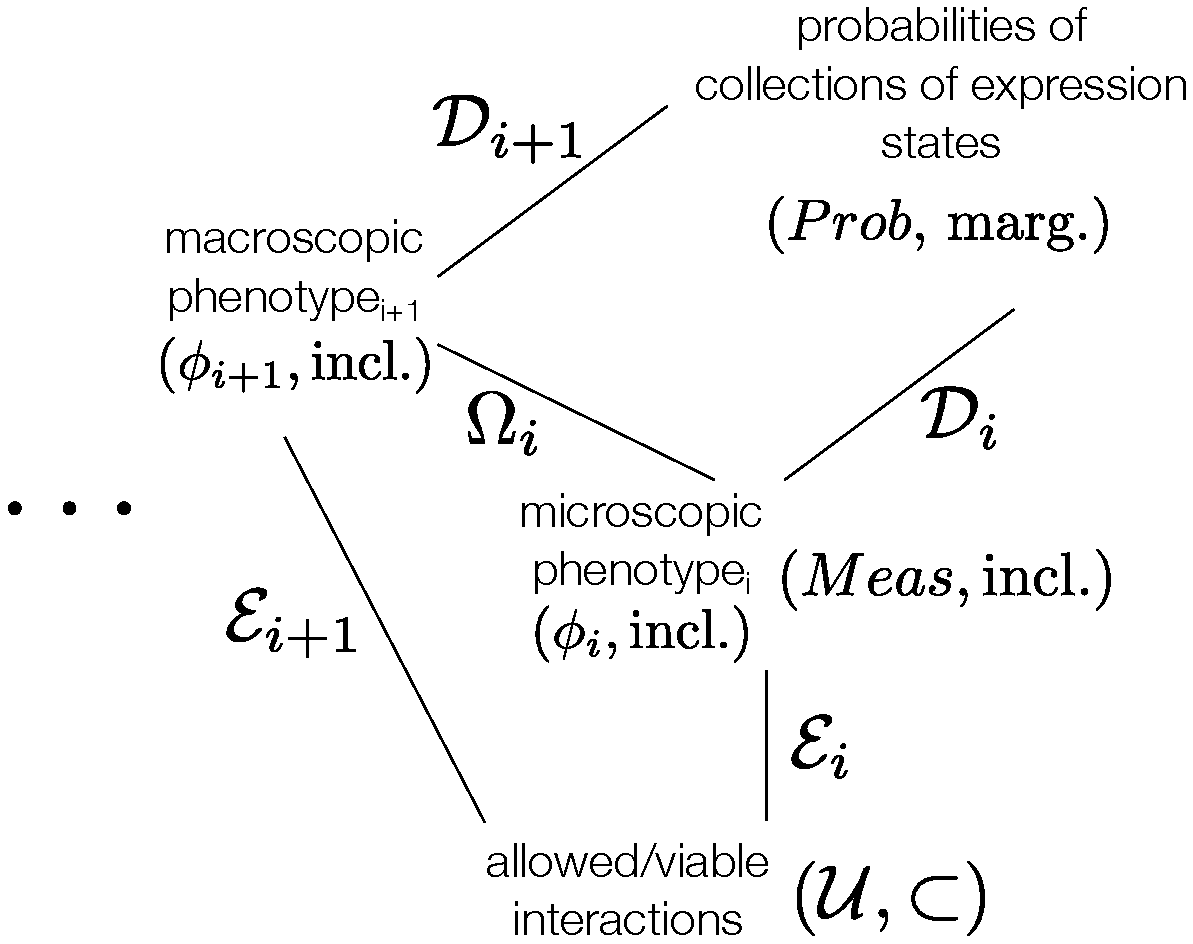
\includegraphics[width=0.4\columnwidth]{fig/abstractroadmap.pdf}
\caption{{\bf Mathematical relationships defining the hierarchy of phenotypes via coarse-graining.} }
\label{fig:abstractroadmap}
\end{figure}

% \pagebreak

% \begin{figure}[!ht]
% \centering
% \noindent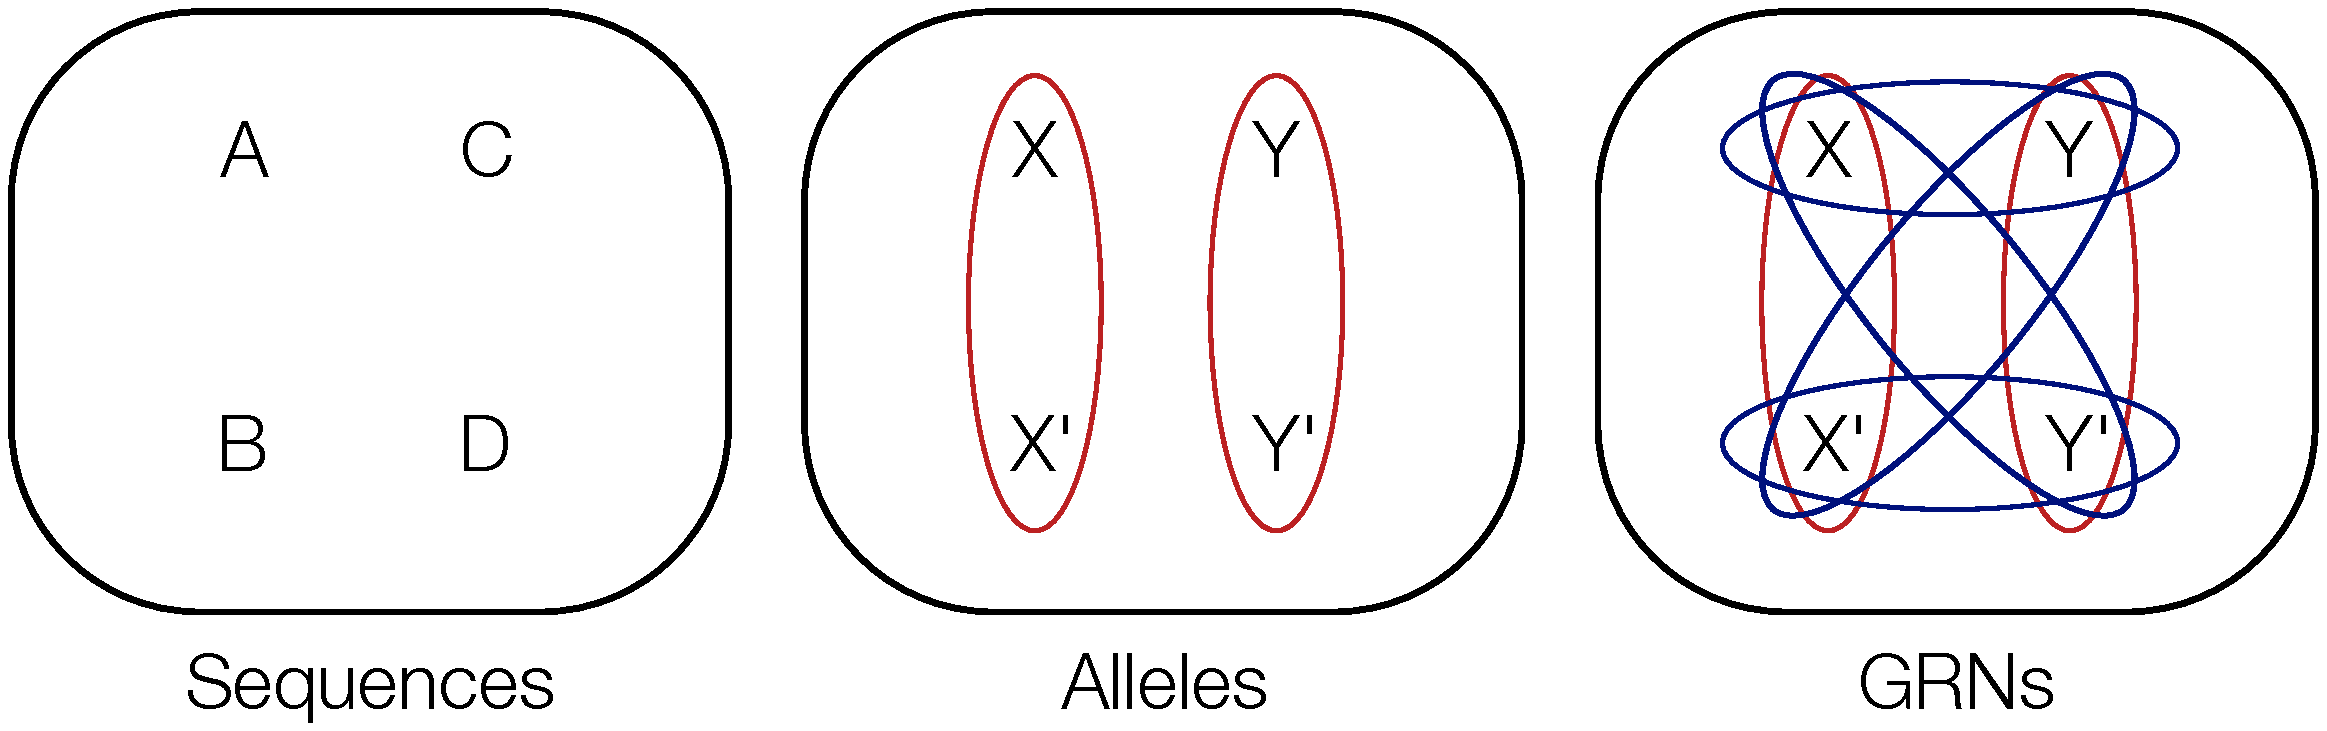
\includegraphics[width=0.7\columnwidth]{fig/genesallelesgrns.pdf}
% \caption{{\bf Sequences, partitions, and GRNs.} In the sequences panel, we consider the letters to be abstract labels for arbitrary genetic sequences that may or may not be found to have a particular function once genetic interactions are taken into account. Sequences may be grouped together, for example if they appear mutually exclusively in gene regulatory networks, under identifications such as~$A=X,\,B=X',\,C=Y,\,D=Y'$. Genomes could then, for example, take one gene from each subset of sequences, by analogy to the partitions representing alleles and the organisms being haploid with all genes are essential. However, in general, we may consider arbitrary subsets of genes to be able to be included in a genome.}
% \label{fig:genesallelesgrns}
% \end{figure}
% \begin{center}
% 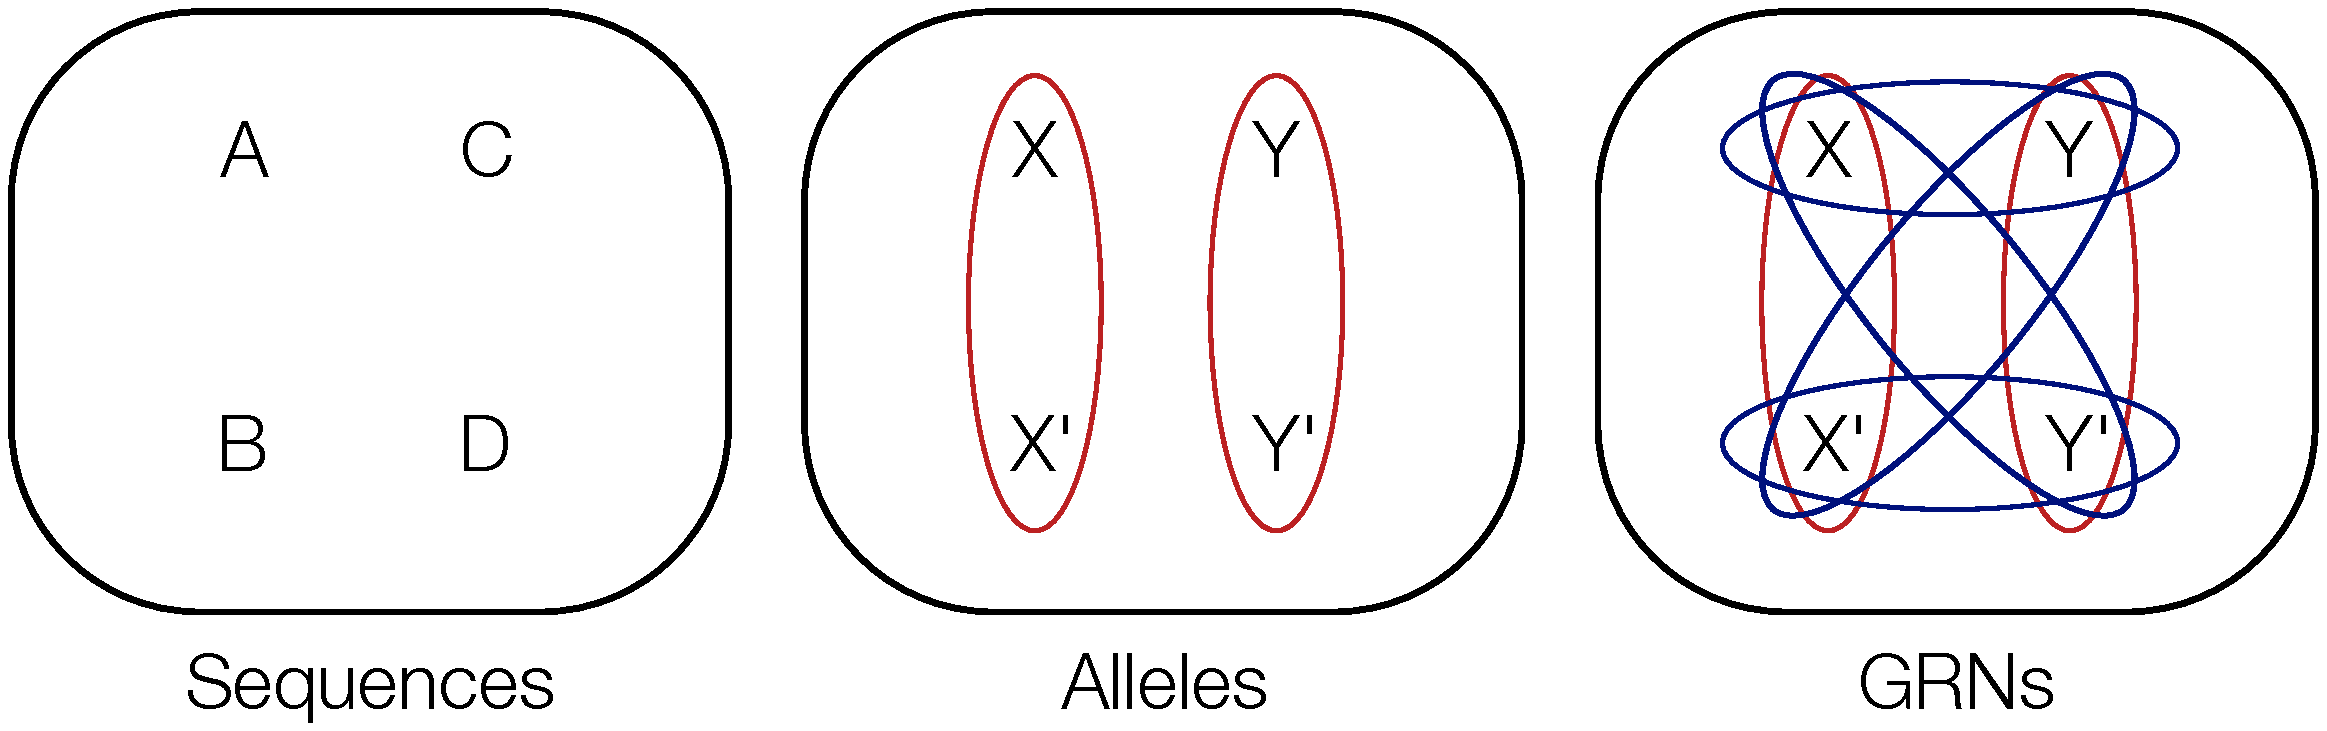
\includegraphics[width=0.9\columnwidth]{fig/genesallelesgrns.pdf}
% \end{center}
% \begin{figure}[!ht]
% \centering
% \noindent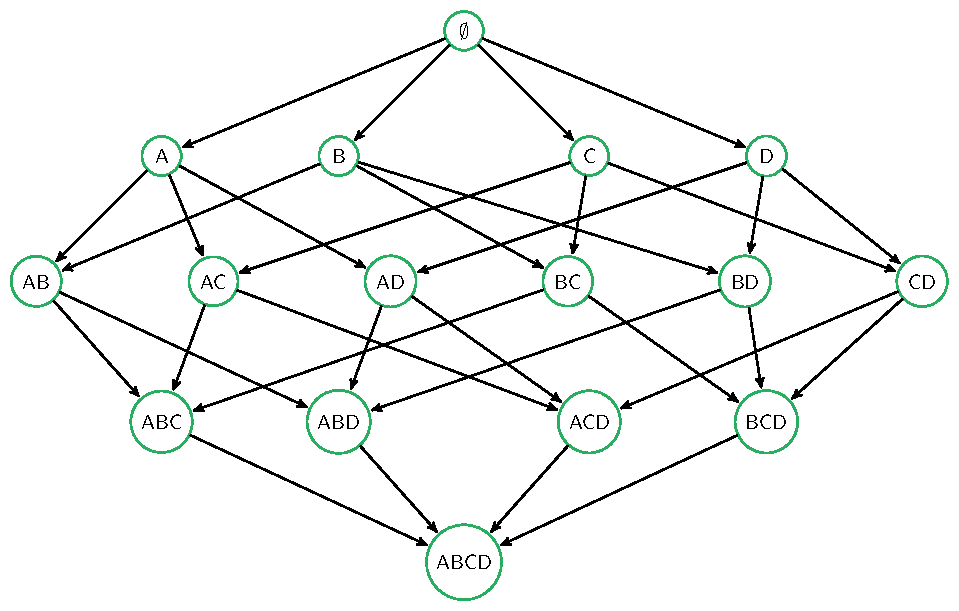
\includegraphics[width=0.4\columnwidth]{fig/potential-interactions.pdf}
% 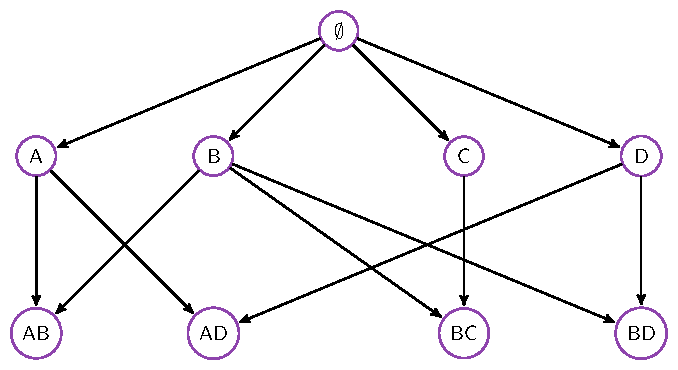
\includegraphics[width=0.4\columnwidth]{fig/two-gene-two-allele-interactions.pdf}
% 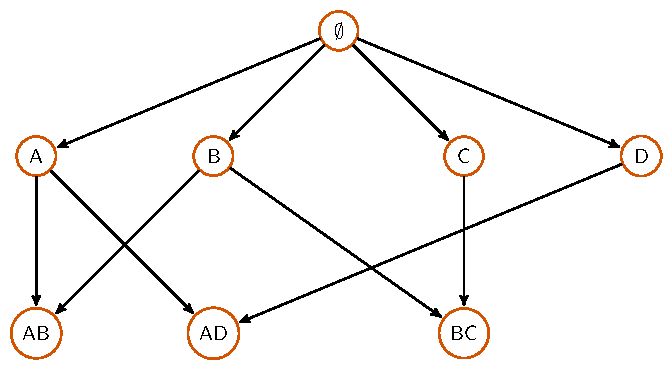
\includegraphics[width=0.4\columnwidth]{fig/incompatibility-interactions.pdf}
% 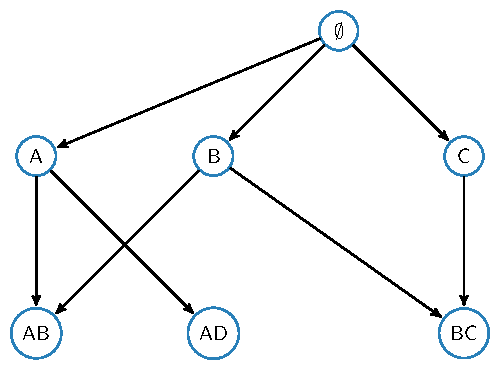
\includegraphics[width=0.4\columnwidth]{fig/dependency-interactions.pdf}
% \caption{{\bf Gene interaction lattices.}}
% \label{fig:geneinteractionlattices}
% \end{figure}
\pagebreak

\begin{figure}[!ht]
\centering
\noindent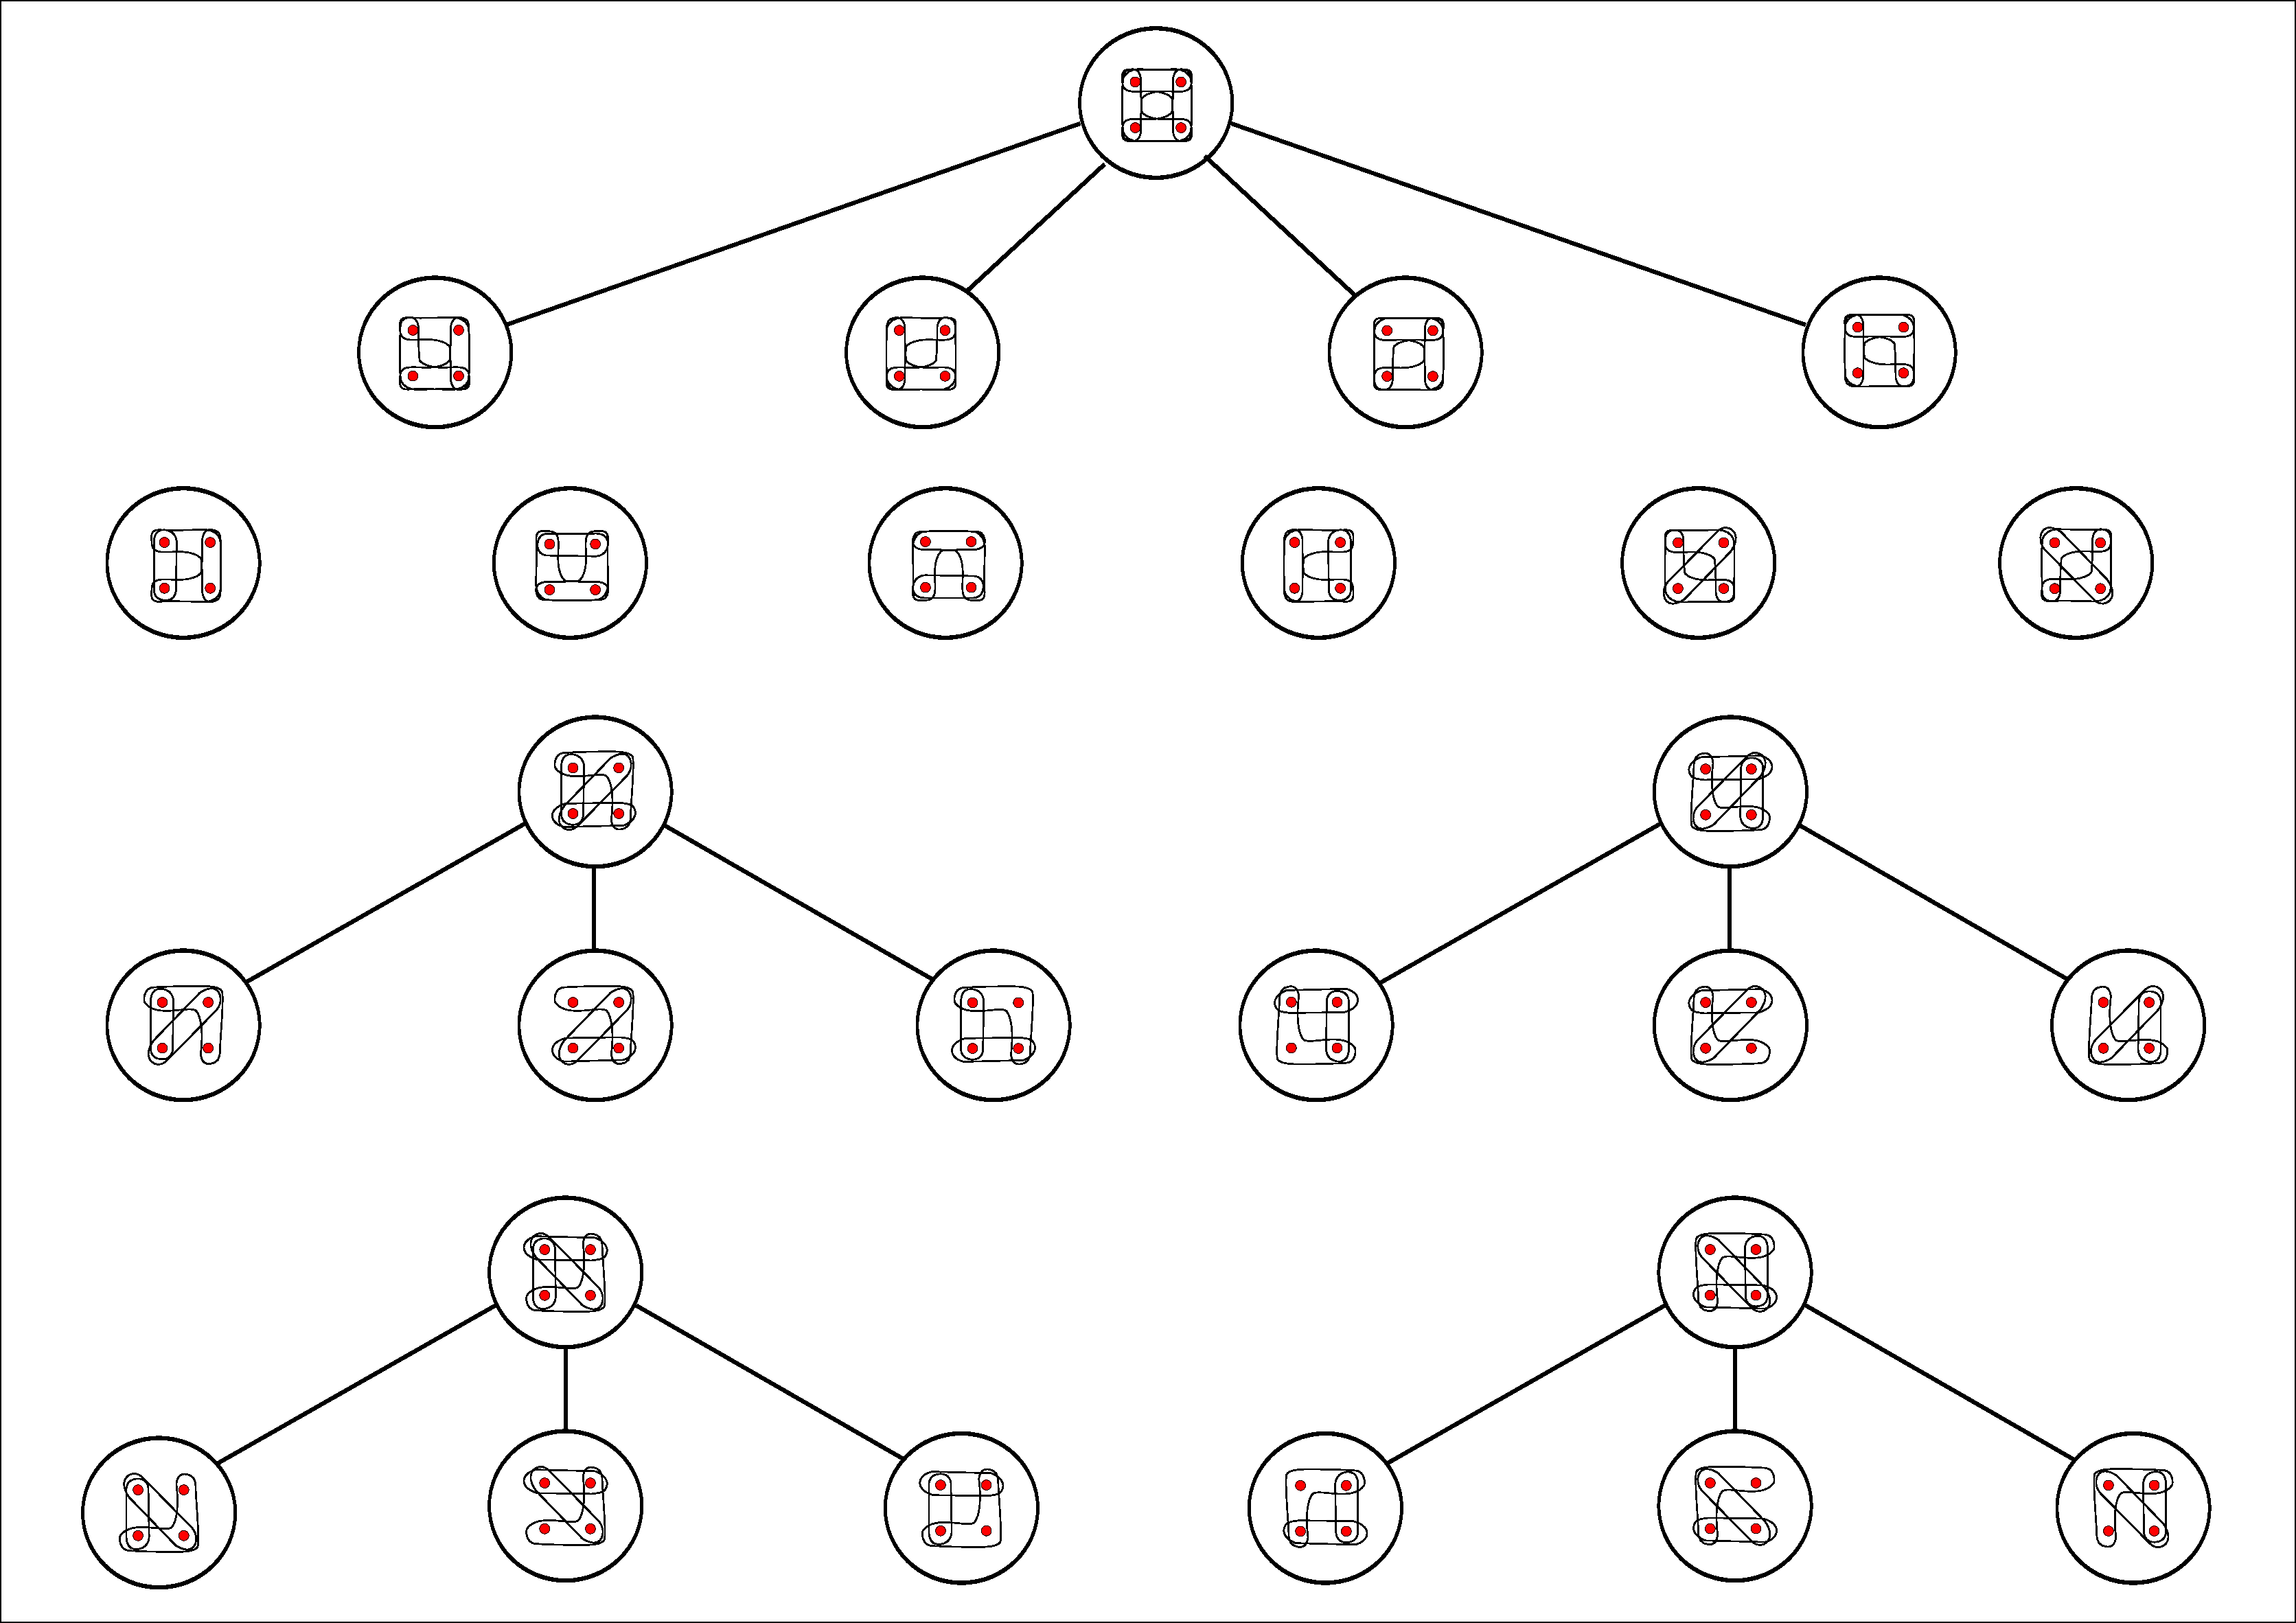
\includegraphics[width=1.0\columnwidth]{fig/non2uniformcyclichypergraphhasse.pdf}
\caption{{\bf Hierarchical relationships among all possible classes of hypergraphs that are not graphs (i.e. not 2-uniform) but have cycles.} (A) There is a Hasse diagram for the lattice of GRNAs analogous to that of \ref{fig:conediagram}A but defined on four rather than only three genes. Within this lattice some of the graphs have cycles and some do not. (B) The highest levels of the Hasse diagram associated to the lattice of GRNAs on four genes containing hypergraphs having cycles. (C) and (D) contain lower levels of GRNAs containing cycles. Each of the four panels in (D) are on the same level. In total, each level represents an isomorphism class of hypergraphs. Therefore, there are five isomorphism classes of non-2-uniform hypergraphs representing GRNAs on four genes that contain cycles leading to the relationship between spaces of probability distsributions on associated genotype-phentoype maps analogous to that of \ref{fig:conediagram}C.}
\label{fig:non2uniformcyclichypergraphhasse}
\end{figure}

% \pagebreak

% \begin{figure}[!ht]
% \centering
% \noindent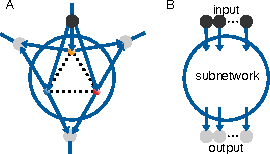
\includegraphics[width=0.3\columnwidth]{fig/controlnetwork.pdf}
% \caption{{\bf Embedding into a particular network context.} The network inside the blue circle is equivalent to that of \ref{fig:inconsistentthreecycle}A, embedded into a particular network context that provides inputs (dark gray node) and outputs (light gray nodes) to the focal subnetwork. As a result of their connectivity, the outputs depend here upon pairwise correlations within the three genes comprising the focal subnetwork.}
% \label{fig:controlnetwork}
% \end{figure}

% \pagebreak

% \begin{figure}[!ht]
% \centering
% \noindent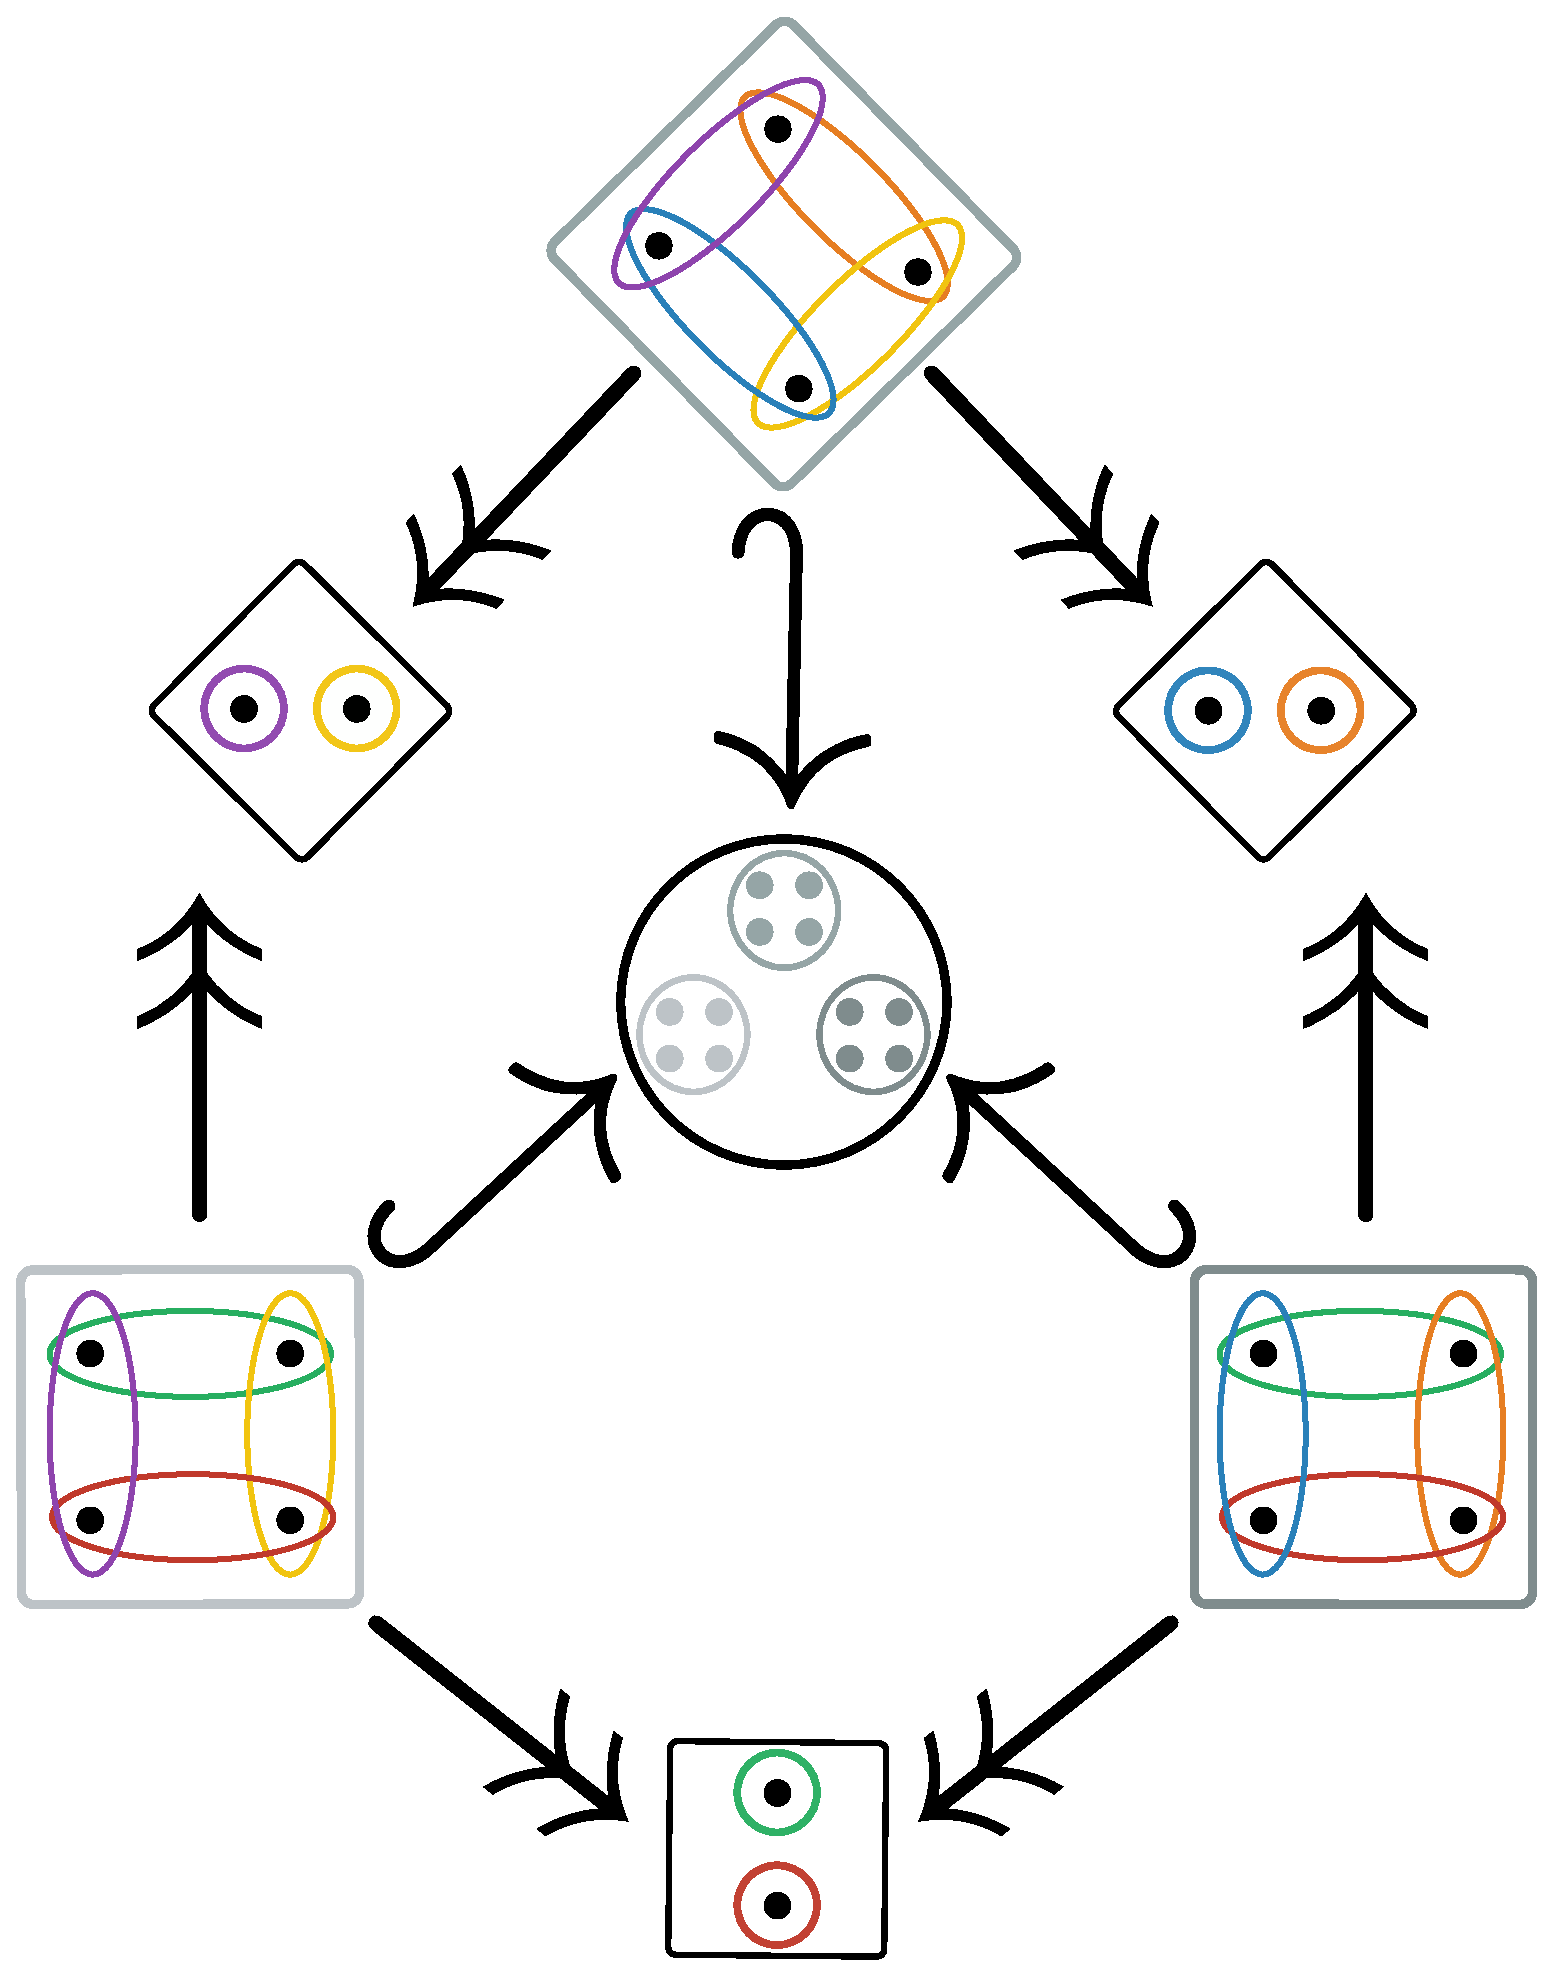
\includegraphics[width=0.5\columnwidth]{fig/condmargprobspaces.pdf}
% \caption{{\bf Diagrammatic representation of the sample spaces for the process generating apparent inconsistency.}}
% \label{fig:condmargprobspaces}
% \end{figure}
